\documentclass[aspectratio=169,11pt]{beamer}
\usetheme{Madrid}
\usecolortheme{default}
\setbeamertemplate{navigation symbols}{}
\usepackage[utf8]{inputenc}
\usepackage[T1]{fontenc}
\usepackage{lmodern}
\usepackage[indonesian]{babel}
\usepackage{graphicx}
\usepackage{booktabs}
\usepackage{array}
\usepackage{tikz}
\usepackage{listings}
\usepackage{xcolor}
\usepackage{multicol}
\usepackage{ragged2e}
\usepackage{adjustbox}
\usepackage{hyperref}
\usepackage{amsmath}
\usepackage{amsfonts}

\graphicspath{{01_Materi/M01_Python_Dasar_Alur_Logika/assets/}{assets/}}

\definecolor{DeepNavy}{HTML}{0B1220}
\definecolor{Navy}{HTML}{12355B}
\definecolor{Blue}{HTML}{1F77B4}
\definecolor{Teal}{HTML}{00A6A6}
\definecolor{Gold}{HTML}{F2B705}
\definecolor{LightBlue}{HTML}{EAF4FF}
\definecolor{LightTeal}{HTML}{E7FAF8}
\definecolor{SoftGray}{HTML}{F4F6F8}
\definecolor{CodeBg}{HTML}{F8FAFC}
\definecolor{DarkText}{HTML}{15202B}
\definecolor{Purple}{HTML}{6F42C1}

\setbeamercolor{title}{fg=white}
\setbeamercolor{frametitle}{fg=white,bg=Navy}
\setbeamercolor{structure}{fg=Blue}
\setbeamercolor{normal text}{fg=DarkText,bg=white}
\setbeamercolor{block title}{fg=white,bg=Navy}
\setbeamercolor{block body}{fg=DarkText,bg=LightBlue}
\setbeamercolor{alerted text}{fg=Gold}
\setbeamerfont{title}{size=\LARGE,series=\bfseries}
\setbeamerfont{subtitle}{size=\large}
\setbeamerfont{frametitle}{size=\large,series=\bfseries}
\setbeamerfont{footline}{size=\fontsize{7.2}{8}\selectfont}
\setbeamertemplate{itemize items}[circle]

\lstdefinestyle{py}{
  language=Python,
  basicstyle=\ttfamily\footnotesize,
  keywordstyle=\color{Blue}\bfseries,
  commentstyle=\color{Teal},
  stringstyle=\color{Gold!70!black},
  showstringspaces=false,
  breaklines=true,
  frame=single,
  rulecolor=\color{Navy!35},
  backgroundcolor=\color{CodeBg},
  tabsize=4,
  columns=fullflexible
}

\newcommand{\mkfooter}{Pemrograman untuk Ilmu Data dan Komputasi}
\newcommand{\prodi}{Program Studi Matematika ITERA}
\setbeamertemplate{footline}{%
\leavevmode%
\hbox{%
\begin{beamercolorbox}[wd=.45\paperwidth,ht=2.35ex,dp=.95ex,leftskip=1.0ex]{author in head/foot}\mkfooter\end{beamercolorbox}%
\begin{beamercolorbox}[wd=.37\paperwidth,ht=2.35ex,dp=.95ex,center]{author in head/foot}\prodi\end{beamercolorbox}%
\begin{beamercolorbox}[wd=.18\paperwidth,ht=2.35ex,dp=.95ex,rightskip=1.0ex plus1fil]{author in head/foot}\hfill\insertframenumber/\inserttotalframenumber\end{beamercolorbox}%
}%
}

\title[\mkfooter]{Pertemuan 1: Mengapa Pemrograman Penting?}
\subtitle{Kontrak Kuliah dan Python Dasar}
\author{Rifky Fauzi dan Triyana Muliawati, S.Si., M.Si.}
\institute{Program Studi Matematika, Institut Teknologi Sumatera}
\date{Ganjil 2026/2027}

\begin{document}

% 1
\begin{frame}[plain]
\begin{tikzpicture}[remember picture,overlay]
\node[anchor=center] at (current page.center){
\includegraphics[width=\paperwidth,height=\paperheight]{tech_bg.png}};
\fill[DeepNavy,opacity=.82] (current page.south west) rectangle ([xshift=8.15cm]current page.north west);

\node[anchor=north west,text=white,align=left,text width=7.0cm] at ([xshift=.65cm,yshift=-.45cm]current page.north west){%
{\fontsize{24}{27}\selectfont\bfseries Pemrograman\\untuk Ilmu Data\\dan Komputasi}\\[3mm]
{\fontsize{15.5}{18}\selectfont Pertemuan 1: Kontrak Kuliah\\dan Python Dasar}\\[2.5mm]
{\fontsize{10.5}{12}\selectfont MA25-21008 \quad Kelas RA dan RB}\\[5mm]
{\fontsize{10}{11.5}\selectfont Rifky Fauzi\\Triyana Muliawati, S.Si., M.Si.}\\[3mm]
{\fontsize{9.3}{10.8}\selectfont Program Studi Matematika\\Institut Teknologi Sumatera\\Semester Ganjil 2026/2027}
};

\node[anchor=north east,fill=white,fill opacity=.95,text opacity=1,rounded corners=3pt,inner sep=4.5mm,text width=7.55cm] at ([xshift=-.38cm,yshift=-.78cm]current page.north east){%
\centering
{\fontsize{13}{15}\selectfont\bfseries Jadwal Mingguan}\\[3mm]
{\fontsize{8.6}{10}\selectfont
\begin{tabular}{>{\bfseries}p{1.45cm}c c c c}
\toprule
Jenis & Kelas & Hari & Waktu & Ruang\\
\midrule
\color{Navy}Kuliah & RA & Jumat & 10.15-11.55 & F212(80)\\
\color{Navy}Kuliah & RB & Senin & 10.15-11.55 & F204(80)\\
\addlinespace[1.2mm]
\color{Teal}Praktikum & RA & Senin & 10.00-12.00 & Lab\\
\color{Teal}Praktikum & RB & Jumat & 10.00-12.00 & Lab\\
\bottomrule
\end{tabular}}
\\[2.5mm]
{\fontsize{7.8}{9}\selectfont\color{DarkText}Lab = Lab. Komputasi Matematika dan Statistika}
};
\end{tikzpicture}
\end{frame}

% 2
\begin{frame}{Peta pertemuan hari ini}
\begin{columns}[T]
\column{.48\textwidth}
\begin{block}{Konteks perkuliahan}
\begin{itemize}
  \item Mengapa pemrograman penting untuk Matematika.
  \item Computational thinking dan keterampilan abad 21.
  \item Mengapa Python relevan untuk data dan scientific computing.
  \item Kontrak kuliah, asesmen, dan project PKM.
\end{itemize}
\end{block}
\column{.48\textwidth}
\begin{block}{Python dasar}
\begin{itemize}
  \item Model mental program Python.
  \item Variabel, input, output.
  \item Tipe data \texttt{int} dan \texttt{float}.
  \item Aritmatika, \texttt{if}, dan perulangan.
  \item Tugas mandiri dan quiz e-learning.
\end{itemize}
\end{block}
\end{columns}
\end{frame}



% 3
\begin{frame}{Buku rujukan utama}
\footnotesize
\begin{tabular}{p{2.75cm}p{4.65cm}p{4.65cm}}
\toprule
\textbf{Buku} & \textbf{Urgensi dalam MK} & \textbf{Bagian SAP yang didukung} \\
\midrule
Miller \& Ranum (2013) & Problem solving, algoritma, data, variabel, control structures, functions, Big-O, recursion, searching, sorting. & Fondasi IndoMS M1-M6 \\
\addlinespace[1mm]
Pine (2019) & Scientific computing: NumPy array, vektor, matriks, sistem linear, dan komputasi numerik. & Komputasi Matematika M3 dan M7 \\
\addlinespace[1mm]
McKinney (2022) & NumPy, pandas, Jupyter, wrangling, visualisasi, workflow data, dan pengantar modeling. & Data analysis/data science M9-M12 \\
\bottomrule
\end{tabular}
\vspace{2.5mm}
\colorbox{LightBlue}{\parbox{.96\linewidth}{\textbf{Keputusan:} Pine tidak diganti. Miller \& Ranum memperkuat algoritma dan Big-O; McKinney menjaga arah data analysis dan data science.}}
\end{frame}

% 3
\begin{frame}{Mengapa pemrograman penting bagi mahasiswa Matematika?}
\begin{columns}[T]
\column{.45\textwidth}
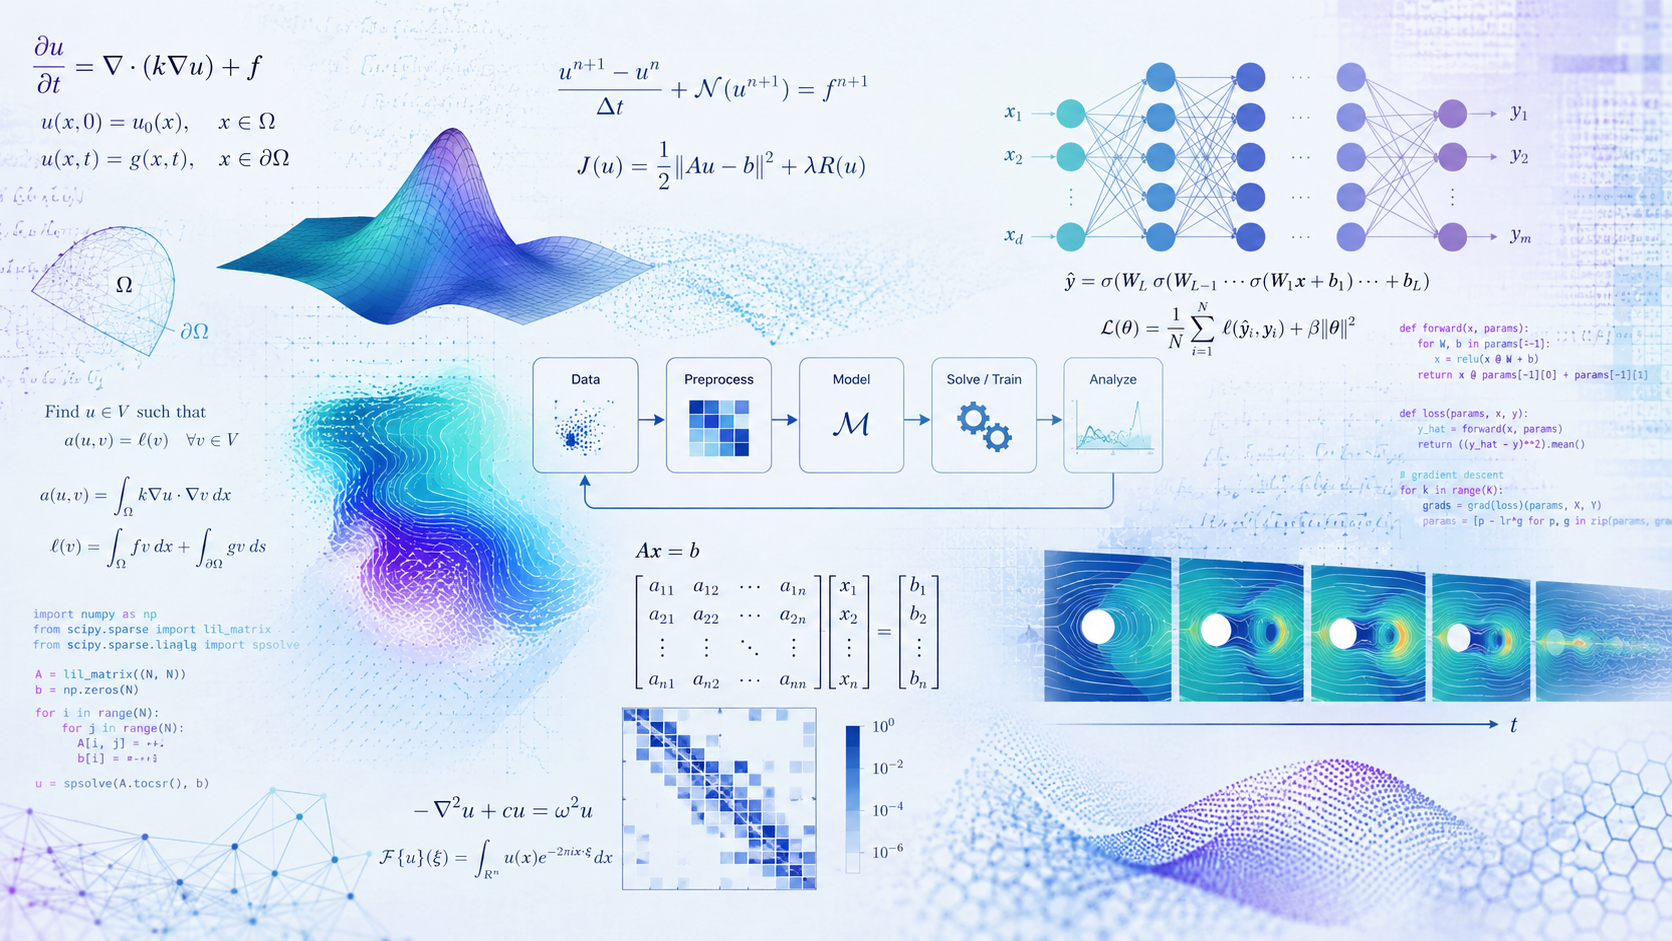
\includegraphics[width=\linewidth]{scicomp_bg.png}
\column{.51\textwidth}
\begin{block}{Matematika memberi struktur}
\begin{itemize}
  \item Variabel, fungsi, matriks, peluang, dan optimisasi.
  \item Asumsi, pembuktian, dan validasi hasil.
  \item Model yang menjelaskan fenomena.
\end{itemize}
\end{block}
\begin{block}{Pemrograman memberi daya eksekusi}
\begin{itemize}
  \item Menguji model pada data nyata.
  \item Menjalankan eksperimen berulang.
  \item Mengubah ide menjadi alat, simulasi, atau analisis.
\end{itemize}
\end{block}
\end{columns}
\end{frame}

% 4
\begin{frame}{Computational thinking dan keterampilan abad 21}
\begin{columns}[T]
\column{.47\textwidth}
\begin{block}{Computational thinking}
\begin{itemize}
  \item Dekomposisi masalah.
  \item Pengenalan pola.
  \item Abstraksi.
  \item Desain algoritma.
  \item Debugging dan evaluasi.
\end{itemize}
\end{block}
\column{.49\textwidth}
\begin{block}{Keterampilan abad 21}
\begin{itemize}
  \item Critical thinking: menilai strategi dan hasil.
  \item Creativity: merancang solusi baru.
  \item Collaboration: membaca dan memperbaiki kode bersama.
  \item Communication: menjelaskan proses, output, dan keterbatasan.
\end{itemize}
\end{block}
\end{columns}
\vspace{1mm}
\footnotesize Rujukan: konsep 4C dari P21; computational thinking dipopulerkan antara lain oleh Jeannette Wing.
\end{frame}

% 5
\begin{frame}{Student-centered learning: bukan dosen tidak mengajar}
\begin{block}{Posisi dosen dan mahasiswa}
\begin{itemize}
  \item Dosen berperan sebagai fasilitator: memberi arah, contoh, tantangan, dan umpan balik.
  \item Mahasiswa aktif membaca, mencoba, salah, memperbaiki, dan menjelaskan ulang.
  \item Sharing sesama mahasiswa adalah bagian dari proses belajar, bukan pengganti dosen.
\end{itemize}
\end{block}
\begin{block}{Mengapa demikian?}
\begin{itemize}
  \item Pemrograman tidak cukup dipahami dengan mendengar penjelasan.
  \item Belajar terbaik terjadi ketika kita mencoba dan menjelaskan kepada orang lain.
  \item Di kelas ini, diskusi dan peer sharing adalah latihan berpikir komputasional.
\end{itemize}
\end{block}
\end{frame}

% 6
\begin{frame}{Manusia, komputer, dan bahasa pemrograman}
\begin{columns}[T]
\column{.52\textwidth}
\begin{block}{Model mental Python}
\centering
\begin{tabular}{c}
Masalah manusia \\
$\downarrow$ \\
Representasi matematika/data \\
$\downarrow$ \\
Algoritma \\
$\downarrow$ \\
Kode Python \\
$\downarrow$ \\
Interpreter + library \\
$\downarrow$ \\
Eksekusi komputer \\
$\downarrow$ \\
Output + interpretasi manusia
\end{tabular}
\end{block}
\column{.44\textwidth}
\begin{block}{Sumber model mental}
Diadaptasi dari Miller \& Ranum (2013) tentang problem solving, algoritma, data, control structures, dan functions; Pine (2019) tentang scientific computing; serta McKinney (2022) tentang Python basics, NumPy, pandas, dan Jupyter.
\end{block}
\end{columns}
\end{frame}

% 7
\begin{frame}{Beberapa simpul sejarah komputasi}
\begin{block}{Tidak satu penemu tunggal}
\begin{itemize}
  \item Charles Babbage: rancangan Analytical Engine.
  \item Ada Lovelace: algoritma untuk mesin Babbage, sering disebut programmer pertama.
  \item Alan Turing: model abstrak komputasi dan batas komputabilitas.
  \item John von Neumann: arsitektur komputer modern dan komputasi numerik.
  \item Grace Hopper: compiler dan bahasa pemrograman yang lebih dekat ke manusia.
\end{itemize}
\end{block}
\vspace{1mm}
\textbf{Pesan:} teknologi komputasi berkembang sangat dekat dengan logika, aljabar, algoritma, statistik, dan pemodelan.
\end{frame}

% 8
\begin{frame}{Perkembangan bahasa pemrograman}
\small
\begin{tabular}{>{\bfseries}p{1.8cm}p{3.2cm}p{7.3cm}}
\toprule
Periode & Bahasa/contoh & Makna perkembangan \\
\midrule
1940-an & Assembly & Dekat dengan instruksi mesin. Cepat, tetapi sulit dibaca. \\
1950-an & FORTRAN, LISP, COBOL & Komputasi ilmiah, simbolik, dan bisnis mulai terstruktur. \\
1970-an & C, Pascal, SQL & Sistem operasi, struktur data, dan basis data. \\
1980-an & MATLAB, C++ & Komputasi matriks dan pemrograman berorientasi objek. \\
1990-an & Python, R, Java, JavaScript & Produktivitas, web, statistik, scripting, dan ekosistem library. \\
2010-an+ & Julia, Rust, Go, Python modern & Performa, keamanan, cloud, AI, data science, dan scientific computing. \\
\bottomrule
\end{tabular}
\vspace{2mm}
\textbf{Inti:} bahasa berubah, tetapi pola berpikir algoritmik tetap bertahan.
\end{frame}

% 9
\begin{frame}{Data terbaru: mengapa Python?}
\begin{columns}[T]
\column{.49\textwidth}
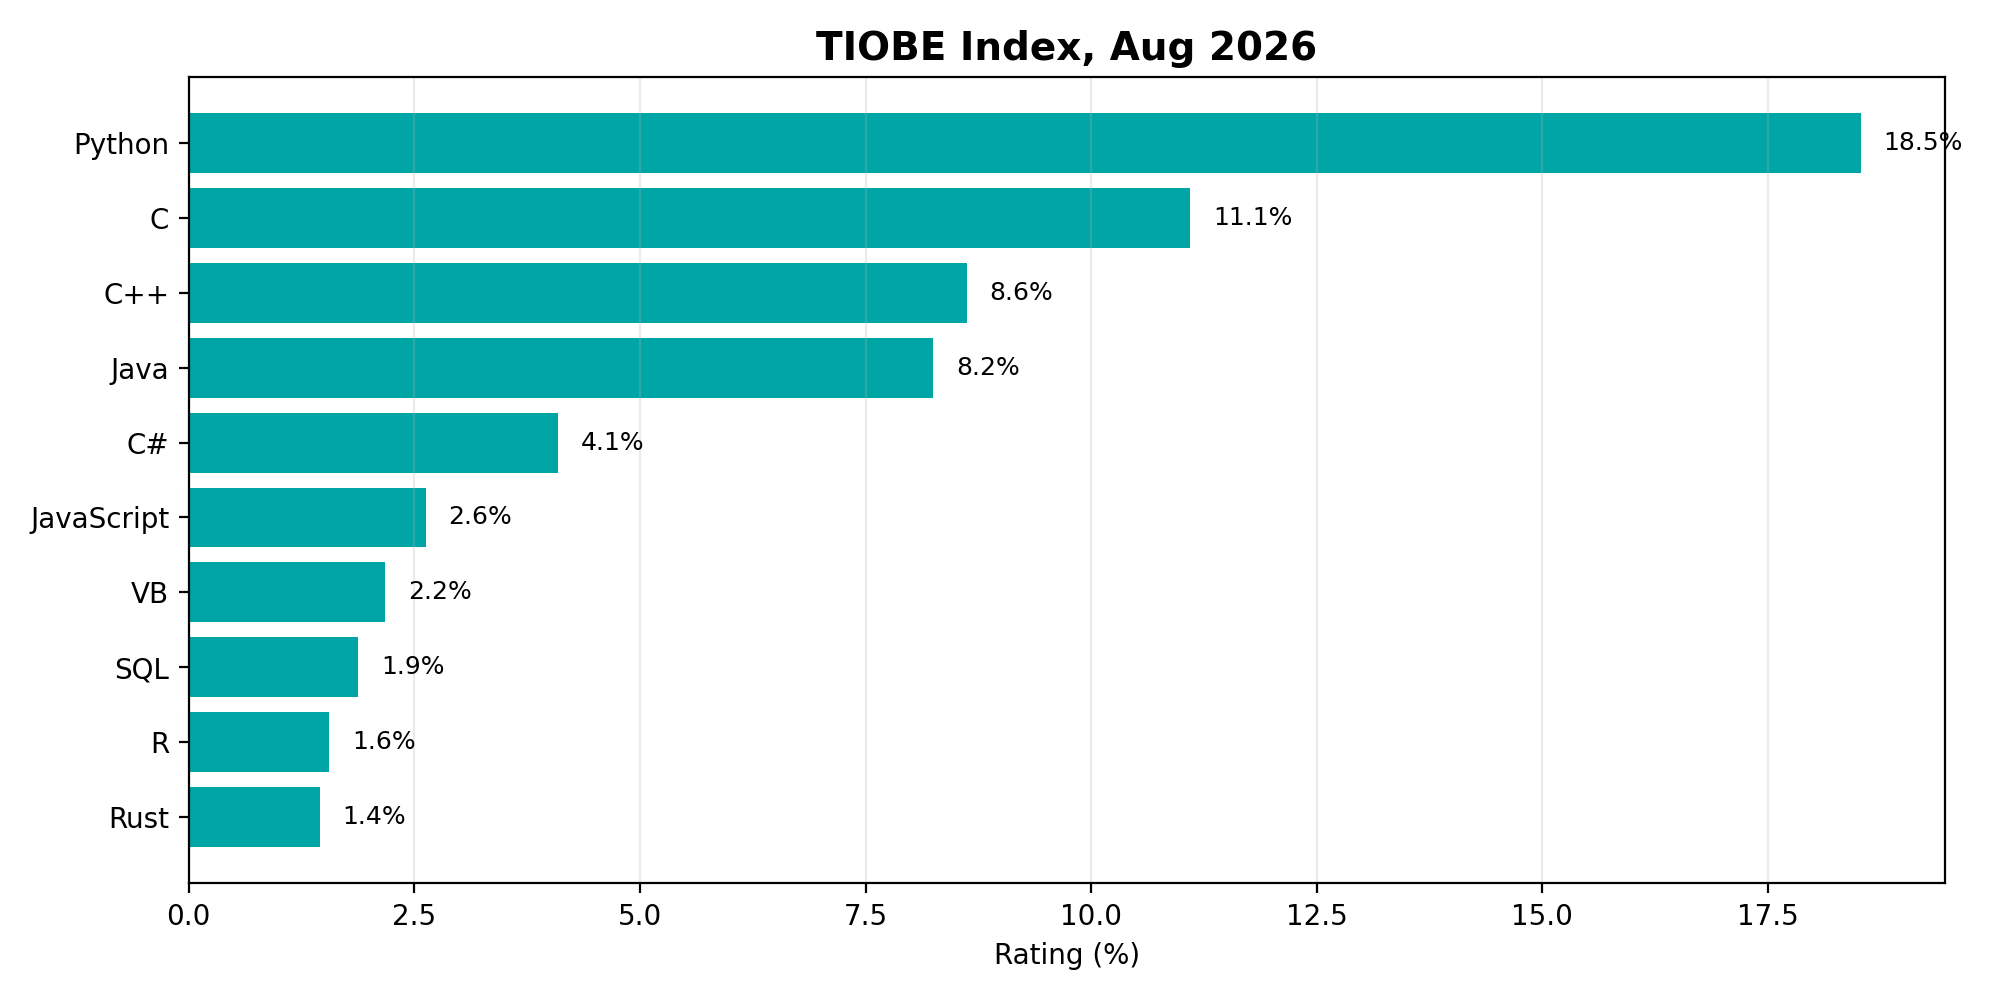
\includegraphics[width=\linewidth]{tiobe_chart.png}
\column{.49\textwidth}
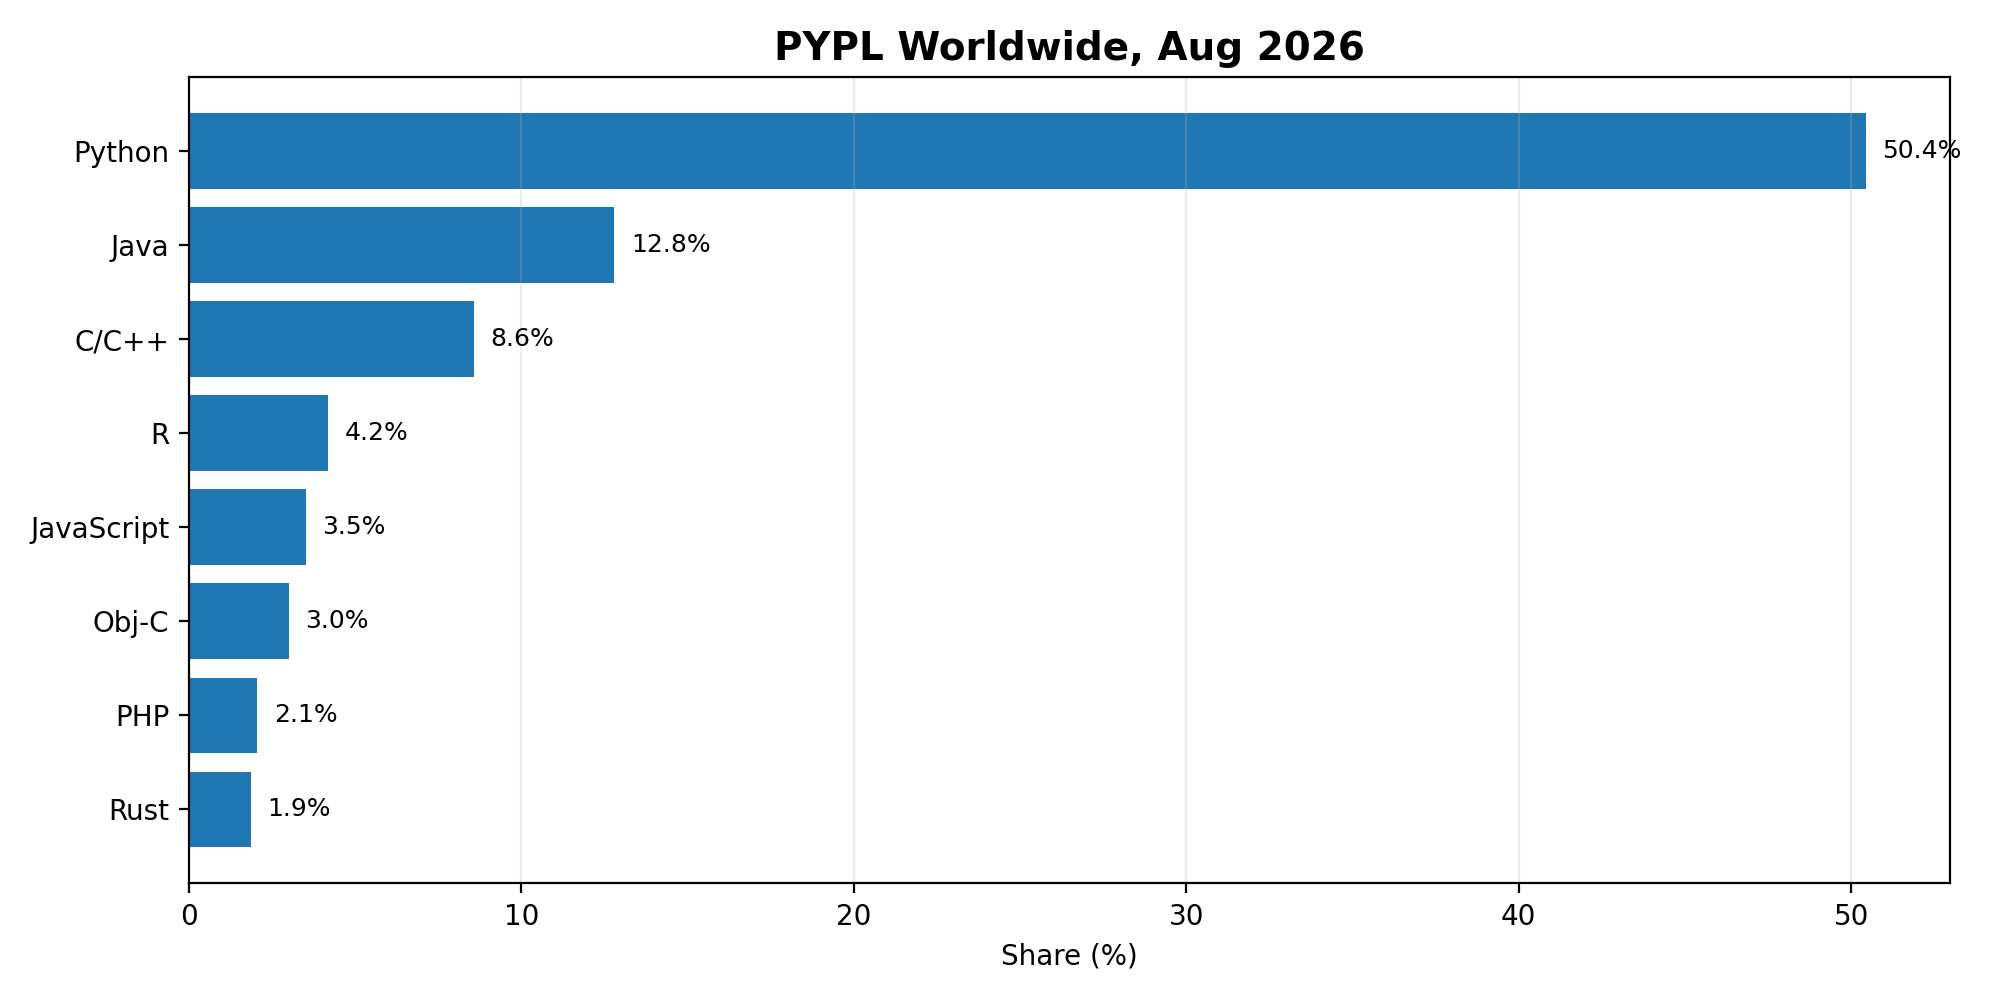
\includegraphics[width=\linewidth]{pypl_chart.png}
\end{columns}
\vspace{1mm}
\footnotesize Sumber: TIOBE Index Aug 2026; PYPL Worldwide Aug 2026. Angka dapat berubah, tetapi pola dominasi Python dalam ekosistem data dan komputasi masih kuat.
\end{frame}

% 10
\begin{frame}{Python di ekosistem developer}
\begin{columns}[T]
\column{.46\textwidth}
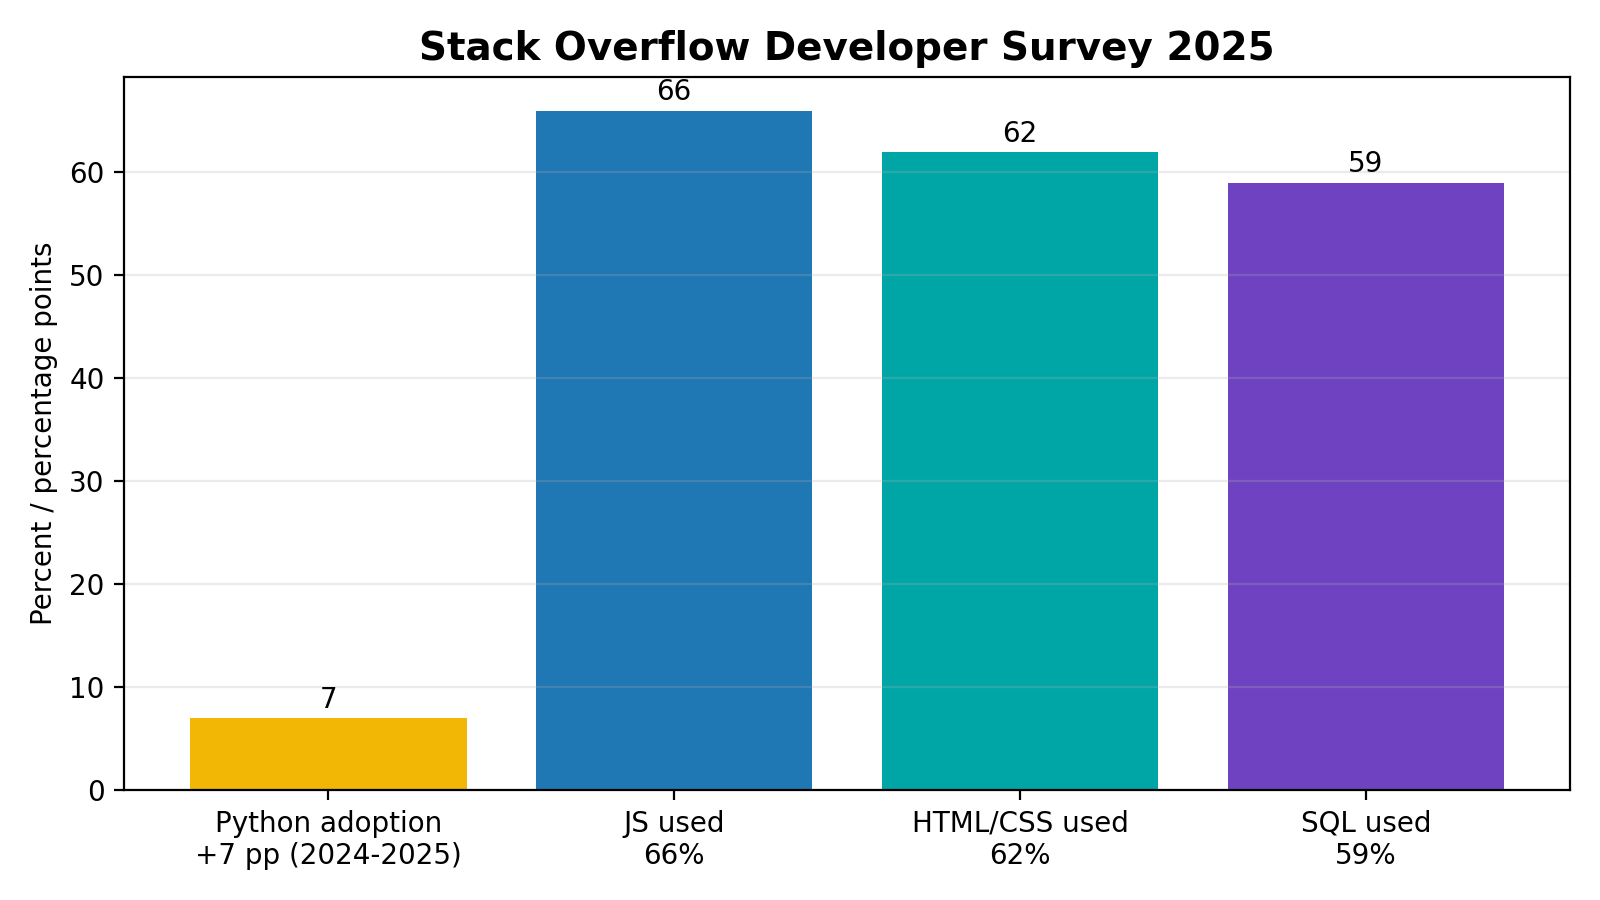
\includegraphics[width=\linewidth]{stackoverflow_chart.png}
\column{.50\textwidth}
\begin{block}{Kekuatan praktis Python}
\begin{itemize}
  \item Sintaks relatif mudah dibaca.
  \item Ekosistem library kuat: NumPy, pandas, matplotlib, SciPy, scikit-learn.
  \item Cocok untuk prototyping, analisis data, model, dan automasi.
  \item Mendukung Jupyter/Google Colab untuk pembelajaran berbasis notebook.
\end{itemize}
\end{block}
\footnotesize Sumber: Stack Overflow Developer Survey 2025 dan dokumentasi ekosistem Python.
\end{columns}
\end{frame}

% 11
\begin{frame}{Ilmu data dan scientific computing untuk lulusan Matematika}
\begin{columns}[T]
\column{.48\textwidth}
\begin{block}{Ilmu data}
\begin{itemize}
  \item Data cleaning dan wrangling.
  \item Statistik deskriptif dan visualisasi.
  \item Regresi, klasifikasi, clustering.
  \item Interpretasi hasil untuk keputusan.
\end{itemize}
\end{block}
\column{.48\textwidth}
\begin{block}{Scientific computing}
\begin{itemize}
  \item Aljabar linier komputasional.
  \item Simulasi numerik.
  \item Analisis algoritma dan eksperimen performa.
  \item Reproducible analysis.
\end{itemize}
\end{block}
\end{columns}
\vspace{2mm}
\textbf{Nilai tambah Matematikawan:} tidak hanya memanggil library, tetapi memahami struktur model, asumsi, dan batas kesimpulan.
\end{frame}

% 12
\begin{frame}{Kontrak kuliah: yang ditekankan}
\begin{block}{Fokus perkuliahan}
\begin{itemize}
  \item Kode Python yang benar, terbaca, dan dapat dijalankan ulang.
  \item Logika algoritmik: urutan langkah, kondisi, perulangan, dan testing.
  \item Data: membaca, merepresentasikan, membersihkan, dan menganalisis.
  \item Project akhir: program Python dan draft proposal PKM.
\end{itemize}
\end{block}
\begin{block}{Sikap belajar}
\begin{itemize}
  \item Aktif bertanya, mencoba, dan berbagi solusi.
  \item Tidak cukup menyalin kode; harus bisa menjelaskan baris penting.
  \item Kesalahan program adalah bahan belajar, bukan aib.
\end{itemize}
\end{block}
\end{frame}

% 13
\begin{frame}{Asesmen dan pembagian minggu}
\small
\begin{tabular}{p{3.5cm}p{2.2cm}p{6.2cm}}
\toprule
Komponen & Bobot & Minggu \\
\midrule
Praktikum & 15\% & M1-M5, M7, M9-M12 \\
Tugas mandiri & 15\% & M1-M5, M7, M9-M12 \\
Quiz e-learning & 10\% & 10 quiz: M1-M5, M7, M9-M12 \\
UTS & 25\% & M8 \\
Final Project: Program Python + Draft Proposal PKM & 35\% & M12-M16: 5\%, 5\%, 7\%, 8\%, 10\% \\
\bottomrule
\end{tabular}
\vspace{2mm}
\begin{block}{Project PKM}
Satu kelompok tugas besar dapat dipisah menjadi dua kelompok saat pengajuan PKM, jika diperlukan untuk menyesuaikan aturan jumlah anggota dan kelayakan ide.
\end{block}
\end{frame}

% 14
\begin{frame}{BAP dan distribusi pengampu}
\small
\begin{tabular}{p{3.5cm}p{3.2cm}p{5.0cm}}
\toprule
Pengampu & Minggu & Fokus \\
\midrule
Triyana Muliawati, S.Si., M.Si. & M2, M3, M7, M9-M12 & Fungsi, NumPy, aljabar linier, regresi, kNN, k-Means, problem framing PKM \\
Rifky Fauzi & M1, M4-M6, M13-M16 & Konsep algoritma, rekursi, Big-O, searching/sorting, analisis kinerja, finalisasi program dan proposal PKM \\
Tim Pengampu & M8 & UTS \\
\bottomrule
\end{tabular}
\vspace{3mm}
\begin{block}{Praktik dan asesmen mingguan}
Praktik, tugas mandiri, dan quiz: M1-M5, M7, M9-M12. Project: M12-M16.
\end{block}
\end{frame}

% 15
\begin{frame}{Project akhir: program Python + draft proposal PKM}
\begin{block}{Alur project}
\begin{itemize}
  \item M12: problem framing, data/mitra, kandidat skema PKM.
  \item M13: studi literatur, metode, dan outline proposal.
  \item M14: demo program Python versi awal dan reproducibility.
  \item M15: draft proposal PKM dan program hampir final.
  \item M16: presentasi final, program Python final, dan draft proposal PKM.
\end{itemize}
\end{block}
\begin{block}{Skema PKM}
Skema tidak dikunci sejak awal. Dosen akan mengarahkan sesuai masalah, data, mitra, dan bentuk solusi.
\end{block}
\end{frame}

% 16
\begin{frame}{Referensi utama: tiga buku, tiga fungsi}
\small
\begin{tabular}{p{2.75cm}p{5.45cm}p{4.6cm}}
\toprule
\textbf{Rujukan} & \textbf{Peran dalam MK} & \textbf{Minggu dominan} \\
\midrule
Miller \& Ranum (2013) & Fondasi IndoMS: problem solving, algoritma, data, variabel, control structures, functions, Big-O, recursion, searching, sorting. & M1-M6 \\
Pine (2019) & Scientific computing: NumPy array, vektor/matriks, komputasi numerik, dan aljabar linier komputasional. & M3, M7 \\
McKinney (2022) & Data analysis/data science: NumPy, pandas, wrangling, visualisasi, workflow data, dan pengantar modeling. & M9-M12 \\
\bottomrule
\end{tabular}
\vspace{2mm}
\begin{block}{Keputusan kurikulum}
Pine tidak diganti. Miller \& Ranum melengkapi bagian algoritma dan Big-O; Pine menjaga identitas scientific computing; McKinney menjaga arah data science.
\end{block}
\end{frame}


% 17
\begin{frame}{Blok komputasi M1-M7: materi dan rujukan}
\scriptsize
\begin{tabular}{p{.7cm}p{7.3cm}p{4.2cm}}
\toprule
\textbf{M} & \textbf{Materi inti} & \textbf{Rujukan utama} \\
\midrule
1 & Konsep algoritma dan pemrograman; data, variabel, pernyataan, operasi, input/output & Miller Ch. 1 \\
2 & Alur logika: sequential, selection, iteration; fungsi dan prosedur secara konseptual & Miller 1.4.3; 1.4.5 \\
3 & Representasi algoritma: narasi, pseudocode, flowchart; list/array dan pengantar NumPy & Miller 1.4.1; Pine NumPy \\
4 & Subprogram, rekursi, base case, recursive case, tracing, dan pengujian sederhana & Miller Ch. 4 \\
5 & Analisis algoritma: $T(n)$, dominant term, Big-O, dan time-space trade-off & Miller Ch. 2 \\
6 & Searching, sorting, dan analisis kinerja algoritma dengan benchmark \texttt{timeit} & Miller 2.3; Ch. 5 \\
7 & Larik multidimensi, vektor, matriks, sistem linear, dan solver komputasional & Pine 9.3 \\
\bottomrule
\end{tabular}
\vspace{1.5mm}
\begin{block}{Catatan IndoMS}
Istilah IndoMS dibuat eksplisit pada SAP: konsep algoritma, representasi algoritma, data/variabel, pernyataan/operasi, alur logika, larik, subprogram, rekursi, dan kompleksitas algoritma.
\end{block}
\end{frame}


% 17
\begin{frame}{Materi Pertemuan 1: Python dasar}
\begin{columns}[T]
\column{.48\textwidth}
\begin{block}{Yang dipelajari}
\begin{itemize}
  \item Variabel dan ekspresi.
  \item Input dan output.
  \item Tipe data \texttt{int} dan \texttt{float}.
  \item Operasi aritmatika.
  \item Kondisional \texttt{if}.
  \item Perulangan \texttt{for} dan \texttt{while}.
\end{itemize}
\end{block}
\column{.48\textwidth}
\begin{block}{Target minimum}
Mahasiswa dapat membuat program/notebook Python yang menerima input sederhana, memproses data numerik, memilih cabang keputusan, dan mengulang proses dengan loop.
\end{block}
\end{columns}
\end{frame}

% 18
\begin{frame}[fragile]{Menjalankan Python: pilih lingkungan kerja yang nyaman}
\begin{block}{Pilihan lingkungan kerja}
\begin{itemize}
  \item Google Colab: praktis melalui browser, tanpa instalasi lokal.
  \item Jupyter Notebook/Lab: cocok untuk komputasi ilmiah dan eksplorasi data.
  \item IDE/editor lokal: VS Code, Spyder, PyCharm, atau editor lain yang mendukung Python.
\end{itemize}
\end{block}
\begin{lstlisting}[style=py]
print("Halo, Matematika ITERA!")
print(2 + 3)
\end{lstlisting}
\end{frame}

% 19
\begin{frame}[fragile]{Variabel dan output}
\begin{columns}[T]
\column{.48\textwidth}
\begin{lstlisting}[style=py]
nama = "Alya"
semester = 3
ipk = 3.45

print(nama)
print(semester)
print(ipk)
\end{lstlisting}
\column{.48\textwidth}
\begin{block}{Model mental}
\begin{itemize}
  \item Variabel adalah nama yang merujuk ke suatu objek/nilai.
  \item Operator \texttt{=} berarti assignment, bukan sama dengan matematis.
  \item \texttt{print()} menampilkan nilai ke layar.
\end{itemize}
\end{block}
\end{columns}
\end{frame}

% 20
\begin{frame}[fragile]{Input dan output}
\begin{columns}[T]
\column{.52\textwidth}
\begin{lstlisting}[style=py]
nama = input("Nama: ")
umur = int(input("Umur: "))

print("Halo", nama)
print("Tahun depan umurmu", umur + 1)
\end{lstlisting}
\column{.44\textwidth}
\begin{block}{Catatan penting}
\begin{itemize}
  \item Hasil \texttt{input()} selalu berupa string.
  \item Gunakan \texttt{int()} atau \texttt{float()} jika perlu angka.
  \item Output harus membantu manusia memahami hasil program.
\end{itemize}
\end{block}
\end{columns}
\end{frame}

% 21
\begin{frame}{Bilangan bulat di komputer: dari desimal ke biner}
\begin{columns}[T]
\column{.47\textwidth}
\begin{block}{Contoh: $13_{10}$}
\[
13 = 8+4+1 = 2^3+2^2+2^0
\]
\[
13_{10}=1101_2
\]
Dalam 8 bit unsigned:
\[
\boxed{00001101_2}
\]
\end{block}
\column{.49\textwidth}
\begin{block}{Bobot setiap bit}
\centering
\begin{tabular}{c|cccccccc}
bit & 7&6&5&4&3&2&1&0\\\hline
bobot &128&64&32&16&8&4&2&1\\
nilai &0&0&0&0&1&1&0&1
\end{tabular}
\end{block}
\begin{block}{Mengapa jumlah bit penting?}
8-bit unsigned hanya punya $2^8=256$ pola: 0 sampai 255. Dengan signed two's-complement: -128 sampai 127.
\end{block}
\end{columns}
\end{frame}

% 22
\begin{frame}[fragile]{Tipe data: \texttt{int} dan \texttt{float}}
\begin{columns}[T]
\column{.50\textwidth}
\begin{lstlisting}[style=py]
a = 7        # int
b = 7.0      # float
c = 2 ** 100 # int besar di Python

print(type(a))
print(type(b))
print(c)
\end{lstlisting}
\column{.46\textwidth}
\begin{block}{Inti konsep}
\begin{itemize}
  \item \texttt{int}: bilangan bulat.
  \item \texttt{float}: bilangan riil aproksimasi di komputer.
  \item Python \texttt{int} dapat sangat besar selama memori cukup.
  \item Di level mesin/NumPy, batas 32-bit dan 64-bit tetap penting.
\end{itemize}
\end{block}
\end{columns}
\end{frame}

% 22
\begin{frame}{Batas bilangan pada komputer}
\small
\begin{tabular}{p{3cm}p{4cm}p{5cm}}
\toprule
Representasi & Contoh rentang & Makna \\
\midrule
\texttt{int32} signed & $-2^{31}$ sampai $2^{31}-1$ & sekitar $-2{,}147{,}483{,}648$ sampai $2{,}147{,}483{,}647$ \\
\texttt{uint32} & $0$ sampai $2^{32}-1$ & sekitar $0$ sampai $4{,}294{,}967{,}295$ \\
\texttt{int64} signed & $-2^{63}$ sampai $2^{63}-1$ & sekitar $\pm 9.22 \times 10^{18}$ \\
\texttt{float32} & maks. sekitar $3.4 \times 10^{38}$ & presisi sekitar 7 digit desimal \\
\texttt{float64} & maks. sekitar $1.8 \times 10^{308}$ & presisi sekitar 15-17 digit desimal \\
\bottomrule
\end{tabular}
\vspace{2mm}
\textbf{Pelajaran:} komputer menghitung dengan representasi terbatas. Matematika ideal, komputer aproksimatif.
\end{frame}

% 24
\begin{frame}[fragile]{Dari $5.75$ ke representasi floating-point}
\begin{columns}[T]
\column{.48\textwidth}
\begin{block}{Langkah biner}
\[
5.75_{10}=101.11_2=1.0111_2\times 2^2
\]
Untuk IEEE-754 float32:
\begin{itemize}
  \item sign: $0$
  \item exponent: $2+127=129=10000001_2$
  \item fraction: $0111000\ldots$
\end{itemize}
\[
\boxed{0\;|\;10000001\;|\;0111000\ldots}
\]
\end{block}
\column{.48\textwidth}
\begin{lstlisting}[style=py]
x = 5.75
print(x)
print(0.1 + 0.2)
print((0.1 + 0.2) == 0.3)
\end{lstlisting}
\begin{block}{Pesan}
Sebagian pecahan desimal tidak punya representasi biner hingga. Karena itu \texttt{float} adalah aproksimasi, bukan bilangan real matematis yang persis.
\end{block}
\end{columns}
\end{frame}

% 25
\begin{frame}{Perangkat bit kecil: fixed-point sebagai alternatif}
\begin{columns}[T]
\column{.49\textwidth}
\begin{block}{Contoh pedagogis Q8.8 (16 bit)}
Simpan 8 bit untuk bagian bulat dan 8 bit untuk pecahan.
\[
5.75\times 2^8 = 1472
\]
\[
1472_{10}=00000101\;11000000_2
\]
Saat dibaca kembali:
\[
1472/256=5.75
\]
\end{block}
\column{.47\textwidth}
\begin{block}{Mengapa relevan dengan komputer lama?}
Pada banyak perangkat 8/16-bit dan game console generasi lama, tidak tersedia unit floating-point cepat. Programmer sering memilih integer atau fixed-point agar komputasi lebih ringan dan perilakunya terkontrol.
\end{block}
\begin{alertblock}{Catatan}
Q8.8 di sini adalah contoh format fixed-point untuk memahami ide representasi; bukan format wajib suatu konsol tertentu.
\end{alertblock}
\end{columns}
\end{frame}

% 24
\begin{frame}[fragile]{Operasi aritmatika}
\begin{columns}[T]
\column{.48\textwidth}
\begin{lstlisting}[style=py]
a = 10
b = 3

print(a + b)  # tambah
print(a - b)  # kurang
print(a * b)  # kali
print(a / b)  # bagi biasa
print(a // b) # bagi bulat
print(a % b)  # sisa bagi
print(a ** b) # pangkat
\end{lstlisting}
\column{.48\textwidth}
\begin{block}{Prioritas operasi}
Urutan umum mengikuti PEMDAS:
\begin{itemize}
  \item Parentheses.
  \item Exponent.
  \item Multiplication / Division.
  \item Addition / Subtraction.
\end{itemize}
\end{block}
\end{columns}
\end{frame}

% 25
\begin{frame}[fragile]{Kondisional \texttt{if}}
\begin{columns}[T]
\column{.50\textwidth}
\begin{lstlisting}[style=py]
nilai = float(input("Nilai: "))

if nilai >= 75:
    status = "Lulus"
elif nilai >= 60:
    status = "Remedial"
else:
    status = "Belum lulus"

print(status)
\end{lstlisting}
\column{.46\textwidth}
\begin{block}{Pola berpikir}
\begin{itemize}
  \item Komputer memilih cabang berdasarkan kondisi logis.
  \item Kondisi bernilai \texttt{True} atau \texttt{False}.
  \item Indentasi menentukan blok program.
\end{itemize}
\end{block}
\end{columns}
\end{frame}

% 26
\begin{frame}[fragile]{Perulangan \texttt{for} dan \texttt{while}}
\begin{columns}[T]
\column{.48\textwidth}
\begin{lstlisting}[style=py]
# for: jumlah pengulangan jelas
for i in range(5):
    print(i)
\end{lstlisting}
\column{.48\textwidth}
\begin{lstlisting}[style=py]
# while: ulang selama kondisi benar
n = 1
while n < 100:
    n = 2 * n
print(n)
\end{lstlisting}
\end{columns}
\begin{block}{Hubungan dengan Matematika}
Perulangan mirip proses iteratif: barisan, metode numerik, simulasi, dan optimisasi semuanya memerlukan ide pengulangan.
\end{block}
\end{frame}

% 27
\begin{frame}{Sebelum kerja kelompok: hal yang biasanya tidak disukai}
\begin{columns}[T]
\column{.48\textwidth}
\begin{block}{Masalah klasik}
\begin{itemize}
  \item Penumpang gratis.
  \item Diam saat diskusi, muncul saat nilai keluar.
  \item Deadline mepet karena tidak ada progres mingguan.
  \item File tercecer dan versi program membingungkan.
  \item Copy-paste kode tanpa paham.
\end{itemize}
\end{block}
\column{.48\textwidth}
\begin{block}{Kesepakatan project}
\begin{itemize}
  \item Ada pembagian tugas dan log kontribusi.
  \item Setiap anggota wajib bisa menjelaskan bagian penting.
  \item Progress M12-M16 harus menunjukkan capaian dan kendala.
  \item Kode harus dapat dijalankan ulang pada lingkungan Python yang disepakati kelompok.
\end{itemize}
\end{block}
\end{columns}
\end{frame}

% 30
\begin{frame}{Tugas mandiri 1}
\begin{block}{Kerjakan mandiri menggunakan Python}
\begin{enumerate}
  \item Buat file/notebook dengan nama: \texttt{Minggu01\_PythonDasar\_Nama}.
  \item Tulis 5 variabel dengan tipe data berbeda.
  \item Buat program menghitung akar persamaan kuadrat sederhana.
  \item Buat program menghitung jarak dua titik.
  \item Tambahkan minimal 5 komentar yang menjelaskan kode.
  \item Kumpulkan file atau tautan sesuai instruksi e-learning.
\end{enumerate}
\end{block}
\vspace{1mm}
\footnotesize Lingkungan kerja bebas: Google Colab, Jupyter, Spyder, VS Code, atau IDE Python lain.
\end{frame}

% 29
\begin{frame}{Referensi dan sumber data}
\footnotesize
\begin{itemize}
  \item Bradley N. Miller dan David L. Ranum. \textit{Problem Solving with Algorithms and Data Structures Using Python}. Release 3.0, 2013.
  \item David J. Pine. \textit{Introduction to Python for Science and Engineering}. CRC Press, 2019.
  \item Wes McKinney. \textit{Python for Data Analysis: Data Wrangling with pandas, NumPy, and Jupyter}. 3rd ed. O'Reilly Media, 2022.
  \item Python Documentation: \url{https://docs.python.org/3/}
  \item NumPy Documentation: \url{https://numpy.org/doc/}
  \item pandas Documentation: \url{https://pandas.pydata.org/docs/}
  \item TIOBE Index Aug 2026; PYPL Worldwide Aug 2026; Stack Overflow Developer Survey 2025.
\end{itemize}
\end{frame}

\end{document}
